% !TeX root = ../main.tex
% !TEX root = ../main.tex
% -*- root: ../main.tex -*-
% -*- program: pdflatex -*-
\chapter{~MRPC~端盖~TOF~离线数据}
原来的端盖~TOF~采用的塑料闪烁体,分东西两部分,每部分单层结构,闪烁体为扇形,光电倍增管垂直耦合,放置于扇形闪烁体的内端。每部分有~48~块。
图~\ref{fig:end-TOF-sigma}~给出了~端盖TOF~的时间分辨。
其中对于~Bhabha~事例样本,时间分辨为~148~ps;对于双~$\mu$~子事例,时间分辨为~110~ps,\cite{zhaoc:2011}。分辨率的不同主要来自不同粒子与探测器材料不同作用的差别,由于~$\mu$~子散射小,击中塑料闪烁体的位置不确定性较小,相比较~Bhabha~事例而言(位置的不确定性以及多次散射效应)非本征的时间分辨贡献较小,因而时间分辨相对较好。
\begin{figure}[!h]
  \centering
  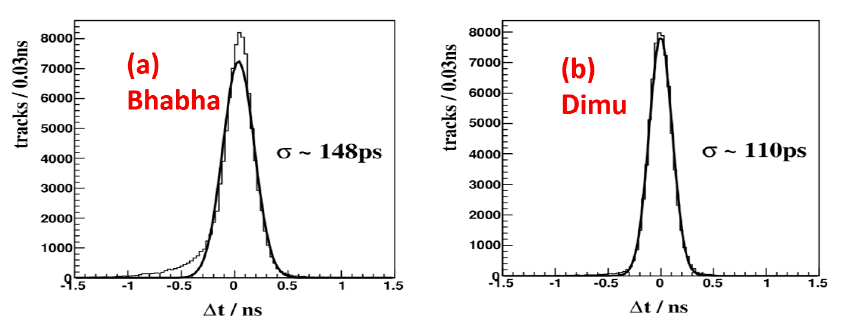
\includegraphics[width=0.9\textwidth]{chap1/end-TOF-sigma.png}
  \caption{端盖~TOF~的时间分辨:(a)电子和(b)~$\mu$~子}
  \label{fig:end-TOF-sigma}
\end{figure}
图~\ref{fig:end-TOF-eff}~给出了端盖~TOF~的各探测单元的效率。探测效率大致为~96$\%$~\cite{wangxz2016}。
\begin{figure}[!h]
  \centering
  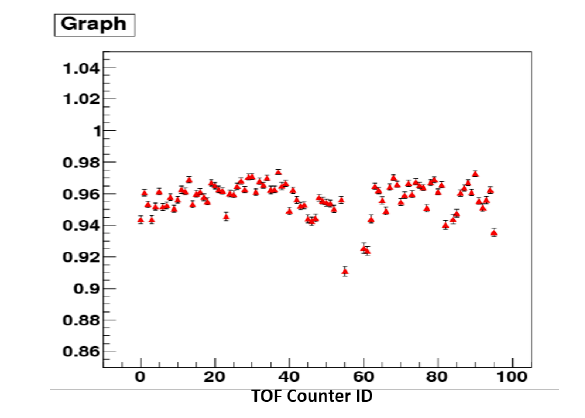
\includegraphics[width=0.8\textwidth]{chap1/end-TOF-eff.png}
  \caption{端盖~TOF~的各探测器单元的效率}
  \label{fig:end-TOF-eff}
\end{figure}

对于端盖~TOF~而言,由于多次散射,导致性能相比较桶部而言,明显较差。~端盖TOF~的~$\pi/K$~的分辨能力如图~\ref{fig:end-TOF-PID}~\cite{zhaoc:2011}所示,在~95.4$\%$(2$\sigma$)~正确率下,$\pi/K$~介子的鉴别能力基本可以达到~1.1~GeV以内。

\begin{figure}[!h]
  \centering
  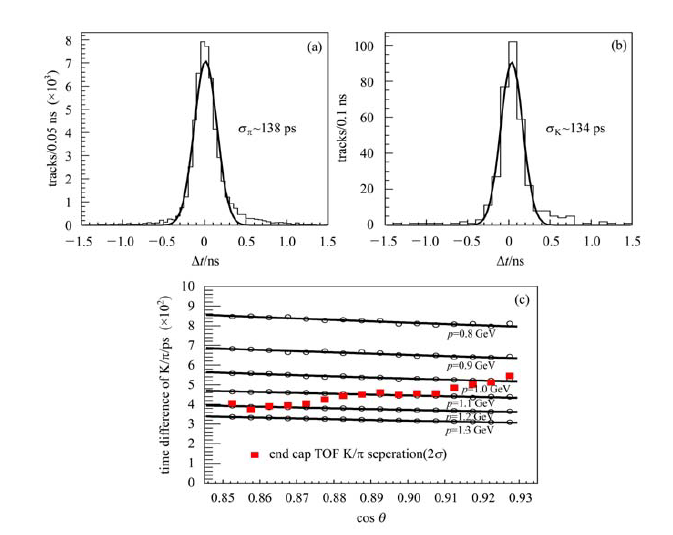
\includegraphics[width=0.9\textwidth]{chap1/end-TOF-PID.png}
  \caption{~1.0~Gev下$\pi$~(a)和~$K$~(b)的时间分辨;(c):端盖~TOF~不同角度下的~$\pi/K$~分辨}
  \label{fig:end-TOF-PID}
\end{figure}

~BESIII~端盖飞行时间探测器采用的是单层的闪烁体结构,以及端盖部分多次散射的影响较大,其本征时间分辨和非本征时间分辨都比较大。

BESIII~谱仪的设计目标是在~$\tau$-粲能区的高精度测量,在这一能区~$J/\psi$~衰变是最主要的物理过程。模拟结果显示,~$J/\psi$~衰变强子动量分布可以达到~1.5~GeV/c,虽然在~0.95~GeV/c以上的强子占的比例较小,但是,对于~BES~物理追求的高精度测量以及稀有衰变事例的研究仍然是非常重要的。因此进一步提高其粒子鉴别能力, 对于提升整个谱仪粒子鉴别能力,完成~BES~物理目标具有重要意义。

测量中性D介子系统的CP破坏和混合参数是~BESIII~的物理目标之一。D介子是唯一没有被测量到~CP~破坏的重味介子。测量D介子混合的黄金衰变道是~$D^0 \to K^- \pi^+$~,~$D^0 \to K^- \pi^+\pi^-\pi^+$~,~$D^+ \to K^- \pi^+\pi^+$~
由于$K$和$\pi$介子的动量分布在~0.8-1.05~GeV,这样我们需要很好的~$\pi/K$~粒子鉴别,要达到较显著的测量结果,要求~$\pi/K$~误鉴别率在~1.05~GeV时要达到~1$\%$~以下。

而~BESIII~目前的端盖~TOF~时间分辨为~140~ps, ~$\pi/K$~的误鉴别率在~1.05~GeV时约为~5$\%$~左右,使得中性D介子的混合参数测量显著性很大程度上下降。由于D介子系统的~CP~破坏很小,粒子物理的标准模型预言~CP~破坏的大小在千分之一左右,要求测量的寻迹系统误差很小,同时也要求~$\pi/K$~的误鉴别应该在~1$\%$~以下。端盖~TOF~的改造不仅改善对带电径迹的粒子鉴别,同时好的飞行时间测量也能提高主漂移室对带电径迹的测量精度,改善寻迹的系统误差,特别是端盖小角度的误差和误鉴别率的改善。当然对于D介子的半轻子衰变和形状因子以及CKM矩阵元Vcs和Vcd的测量,改造后的~TOF~端盖会降低由于粒子误鉴别造成的本底,提高这些物理量的测量精度。 

\section{MRPC~硬件和电子学}
\subsection{端盖MRPC的结构}
升级后的端盖~TOF~采用了~MRPC~技术。利用~MRPC~做成的飞行时间探测器有好的时间分辨,同时又能保证探测效率,有好的粒子鉴别能力,而且价格也便宜。从~MRPC~探测原理出发分析,当带电粒子穿过~MRPC~时,其原初电离的发生雪崩放大现象,这一过程是在多个气隙中同时进行,总的信号等于各个气隙的信号的叠加。因此~MRPC~性能的重要的指标参数是气隙的宽度和数目。采用较小的气隙宽度可以降低工作电压,提高工作稳定性;采用多气隙数目,可以增加带电粒子在气隙中发生雪崩现象的概率,继而可以提高探测效率;可以减小雪崩过程的统计涨落,有利于提高时间分辨。

采用~MRPC~的端盖~TOF~的具体阵列设计如图~\ref{fig:MRPC-TOF}~所示,每层~18~个模块,采用双层结构,通过相邻模块间的交叠可以减少死区,提高探测效率。
\begin{figure}[!h]
  \centering
  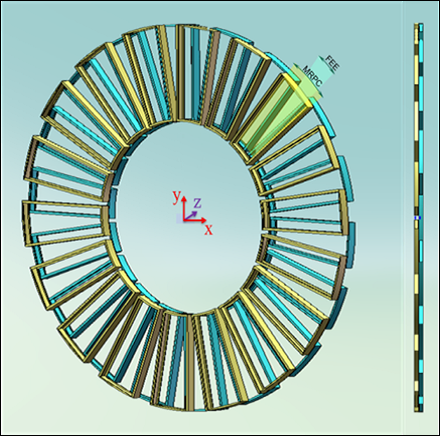
\includegraphics[width=0.5\textwidth]{chap1/MRPC-TOF.png}
  \caption{BESIII/端盖TOF 双层MRPC阵列结构示意图}
  \label{fig:MRPC-TOF}
\end{figure}

每个模块的~PCB~的设计如图~\ref{fig:PCB}~所示。每个模块采用梯形结构,共有~12~个读数条,读数条宽~2.4~cm,相邻读数条之间的距离为~3~mm。读数条最短的是~9.1~cm,最长的是~15.1~cm。每个读数条采用双端读出,共有~24~路读出信号通道。

\begin{figure}[!h]
  \centering
  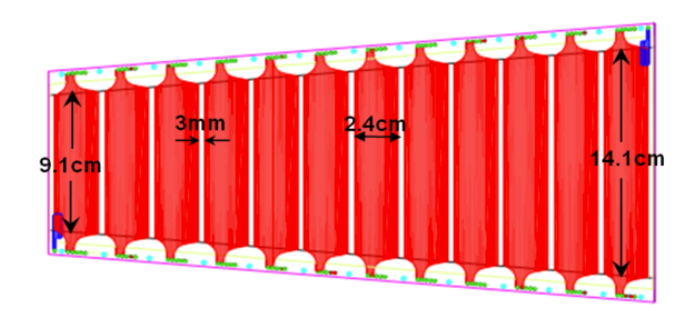
\includegraphics[width=0.9\textwidth]{chap1/PCB.png}
  \caption{MRPC结构示意图}
  \label{fig:PCB}
\end{figure}

MRPC~模型几何结构如图~\ref{fig:MRPC}~所示。模块采用双层堆叠的设计方式,一共有~2*6~个气隙,每个气隙~220~$\mu$m,每个模块的厚度$<$2.4~cm, 双层总厚度$<$5~cm;环状探测器外半径为~844~mm,内半径为~454~mm。
\begin{figure}[!h]
  \centering
  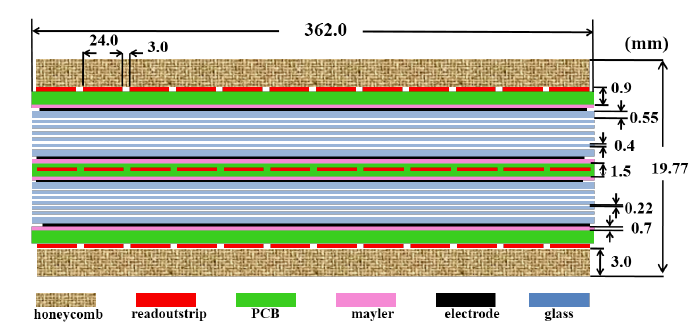
\includegraphics[width=0.9\textwidth]{chap1/MRPC.png}
  \caption{端盖TOF 升级MRPC 的结构图}
  \label{fig:MRPC}
\end{figure}

MRPC~需要工作在气密的环境下,工作气体组分是90$\%$~Freon+5$\%$~S$F_{6}$+5$\%$~iso-$C_{4}H_{10}$。
\subsection{电子学系统}

MRPC~的电子学系统设计方案和电子学系统包含前端放大甄别~FEE(Front end Electronics)模块、飞行时间测量~TDIG(Time to Digital module)插件、提供阈值和电源给~FEE~模块并传输击中信息至触发系统等功能的~CTTP(Coincidence Test Threshold Power module)插件,时钟扇出插件硬件系统和数据获取软件和控制软件系统。

整个系统共~72~个~FEE~模块,FEE~模块采用基于~TOT~技术的~NINO~芯片,每个~FEE~模块含有~4~片~NINO~芯片,产生~24~路LVDS电平的输出信号,共完成~1728~路信号的放大甄别。
MRPC~输出的电荷约为几十fC, 信号脉冲上升时间小于1ns,输出信号电流比较小,必须进行进一步的放大和成形。为了最大程度的利用~MRPC~自身产生的差分信号,~NINO-ASIC~芯片采用差分的输入,全线路的差分信号处理方式。NINO~对输入的信号进行快速放大,同时为了满足过阈时间(TOT)的测量将输入的信号电流转换为了输出的信号宽度。
飞行时间数字化插件~TDIG~。前端电子学输出的信号使用~HPTDC~芯片接收并数字化,并根据数据格式进行打包,经~VME~总线上传至数据获取系统。~NINO~配合~HPTDC~同时测量出信号过阈时间的前沿时间(leading edge)和后沿时间(trailing edge)。其中前沿时间用来定时,结合前沿时间和后沿时间的~TOT~用来修正过阈时间不同引起的时间晃动。
端盖~TOF~电子学系统中,~CTTP~插件共两块,一个~CTTP~插件对应~36~个~FEE~模块。插件的作用是接收~NINO~芯片产生的击中信息,然后通过光纤上传到触发系统;为~NINO~芯片提供阈值电压,电源和测试信号,使芯片正常运行和满足测试需求。~CTTP~插件同时还完成快控制功能。
时钟扇出插件为~TDIG~和~CTTP~插件提供同步时钟信号。

\section{~BESIII~离线数据处理和分析系统}
BESIII~实验开发的一套由软件平台、模拟、刻度、重建和物理分析工具等部分组成的软件系统是为了用来处理和分析~BESIII~离线数据。对探测器和模拟产生的原始数据进行离线处理,生成包含末态粒子各种信息的数据(DST数据)供物理分析使用是它的主要任务,同时连接探测器和物理分析的衔接系统,提供了物理研究所需的各种软件工具。~BESIII~的简化的离线数据处理过程如图~\ref{fig:BESIII-data-flow}~所示。
\begin{figure}[!h]
  \centering
  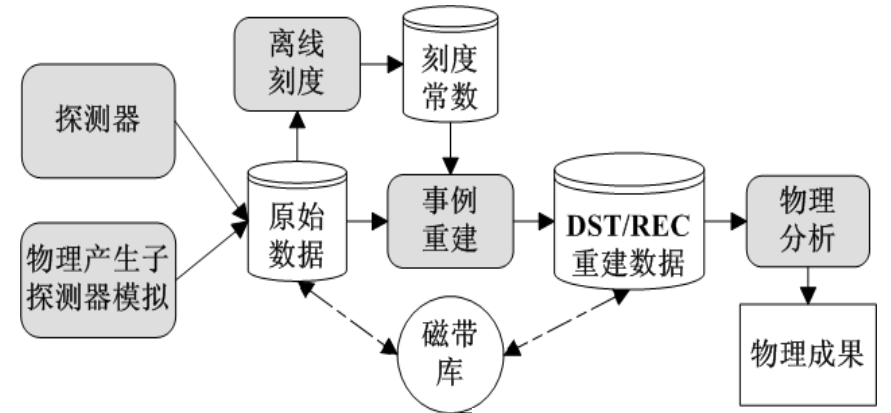
\includegraphics[width=0.9\textwidth]{chap1/BESIII-data-flow.png}
  \caption{简化的BESIII离线数据处理和物理分析过程}
  \label{fig:BESIII-data-flow}
\end{figure}

结合~BESIII~实验的具体需求,选用~cern~的~LHCb~实验开发的通用高能物理实验底层软件框架~GAUDI~~\cite{Barrand:2000}为基础,以C++语言为主要程序语言开发的全新离线数据处理和分析软件平台~\cite{liwd:2006}(BOSS)是~BESIII~离线软件系统的核心部分。

包括离线数据刻度、事例重建、事例分类、MC模拟和物理分析等阶段的离线数据处理的数据管理工具是由BOSS~软件平台提供的。软件平台结合数据处理各阶段的特点和探测器特点的设计出符合不同探测器的数据结构,然后对这些数据采用专门的数据管理服务进行关键。BOSS~软件平台实现动态库的链接机制,可以有效的缩短再编译的时间。软件系统同时采用了如ROOT~\cite{root},CERNLIB~\cite{cern}等国际高能物理实验室的开源软件库和各种软件工具。

图~\ref{fig:BESIII-software}给出了BESIII离线软件平台的整体结构图。软件的核心部分是:模拟、刻度、重建和物理分析算法。
\begin{figure}[!h]
  \centering
  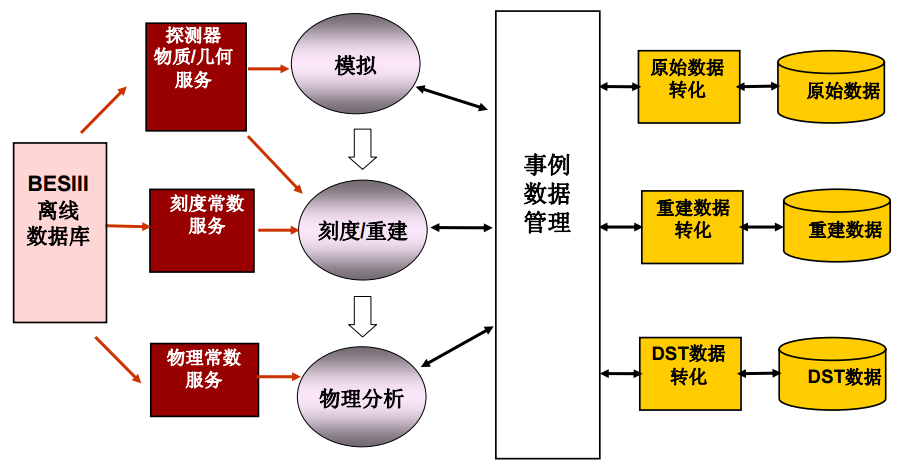
\includegraphics[width=0.9\textwidth]{chap1/BESIII-software.png}
  \caption{BESIII离线软件平台}
  \label{fig:BESIII-software}
\end{figure}

BESIII~数据处理和物理分析软件系统,有超过200个的软件单元。组织和管理这些单元采用的是软件包的形式。BESIII~规范软件开发和发布过程利用的是配置管理工具(Configuration Management Tool,CMT),该工具有一套管理规则和管理工具组成。%【9】

\section{端盖~TOF~数据刻度重建流程}
MDC、EMC、TOF~和~MUC~子系统以及径迹外推和匹配部分组成共同组成~BESIII~离线事例重建软件系统。BEPCII~采用的多束团对撞的机制,BEPCII~的高频时钟为~499.8~MHz,周期为~2~ns,储存环中共有~93~个束团,两个相邻束团之间的时间间隔为~6~ns。BESIII~触发系统的周期为~24~ns,因此在每个触发周期内有~4~个束团对撞,准确的事例起始时间无法由在线系统直接给出。必须通过离线数据分析,通过事例重建,主要是MDC径迹重建,得到最可几事例起始时间。

事例重建系统的一般流程如图~\ref{fig:reconstruction}~。

\begin{figure}[!h]
  \centering
  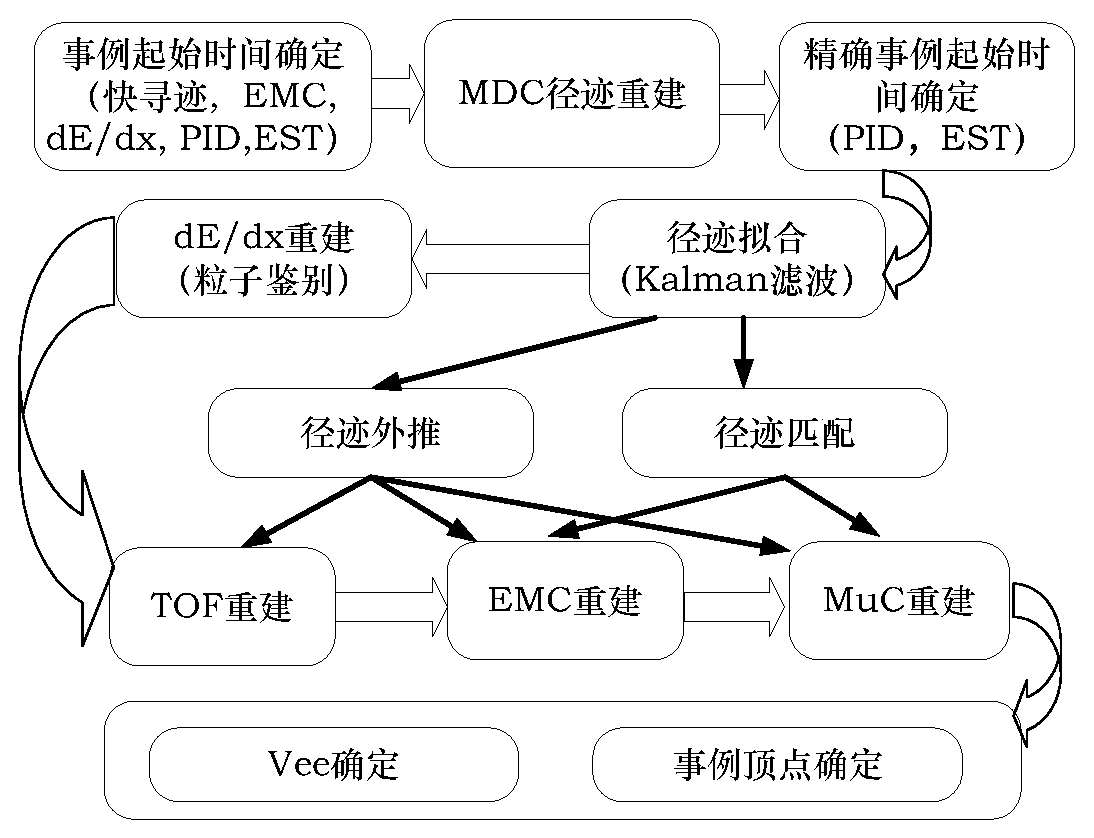
\includegraphics[width=0.7\textwidth]{chap1/reconstruction.eps}
  \caption{BESIII事例重建过程}
  \label{fig:reconstruction}
\end{figure}

\subsection{事例起始时间重建}

前面提到在一个触发周期内有~4~个束团发生对撞,因此准确的事例起始时间无法由在线系统直接给出。事例起始时间需要离线数据重建得到。图~\ref{fig:BESIII-time-system}给出了~BESIII~的时间测量系统。事例的起始时间~$T_{est}$~可以表示为:$T_{est}$=$T_{DCM}$-$T_{ev}$。其中~$T_{est}$~表示事例起始时间,为对撞发生时刻的时间;~$T_{DCM}$~表示~TOF~电子学测量到的原始~TDC~时间,$T_{ev}$~为带电粒子从对撞顶点飞到到给出信号的探测器之间的飞行时间。
\begin{figure}[!h]
  \centering
  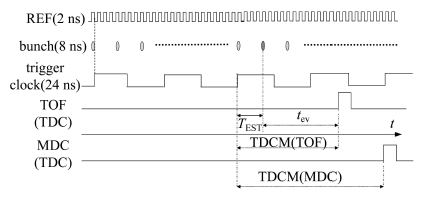
\includegraphics[width=0.6\textwidth]{chap1/BESIII-time-system.png}
  \caption{BESIII事例的时间关系}
  \label{fig:BESIII-time-system}
\end{figure}

图~\ref{fig:Test}~给出了计算事例起始时间~$T_{est}$~的程序流程图。主要包括快重建~\cite{zhangxm:2005}和时间起始时间重建两部分~\cite{max:2007}。在~MDC~快重建和粒子鉴别完成后,$T_{est}$~由~MDC~和~TOF~分别计算得到,具体的计算方法见文献~\cite{Maxiang:2008}。其中~TOF~得到的~$T_{est}$~精确度高。

\begin{figure}[!h]
  \centering
  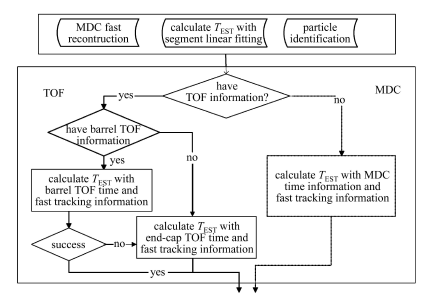
\includegraphics[width=0.6\textwidth]{chap1/Test.png}
  \caption{事例起始时间程序流程图}
  \label{fig:Test}
\end{figure}
\subsection{主漂移室的径迹外推}

~BESIII~主漂移室重建径迹的外推算法,利用小步长外推提供了主漂移室中的带电径迹外推到外部飞行时间探测器,电磁量能器等其他子探测器上的预期径迹信息。算法在外推的过程中充分考虑了带电径迹在磁场中的偏转情况以及带电粒子与探测器物质发生相互作用引起的电离能损等效应, 计算径迹参数的参数误差矩阵时考虑了库仑多次散射效应的影响。

在考虑带电粒子的磁场偏转,以及电离能损的情况下,小步长外推是比较精确的计算径迹的预期参数的一个常用方法。此方法认为径迹可以近似为螺旋线, 在每个小步长外推结束时,从带电粒子的动量中减去该步长的电离能损,之后再进行下一个小步外推,如此直到推至要求的位置~\cite{wangll:2014}。
具体径迹外推程序~TrkExtAlg~流程图见图~\ref{fig:TrkExtAlg}。

\begin{figure}[!h]
  \centering
  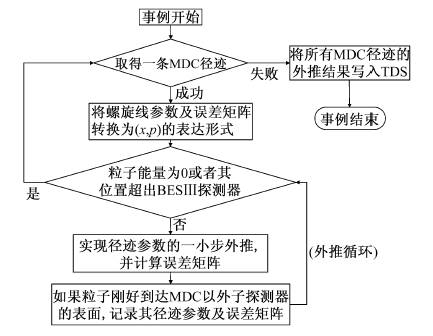
\includegraphics[width=0.6\textwidth]{chap1/TrkExtAlg.png}
  \caption{径迹外推算法的实现流程图}
  \label{fig:TrkExtAlg}
\end{figure}

\subsection{飞行时间探测器的重建}
TOF~离线数据重建流程如图~\ref{fig:TOF-res}~所示。
TOF~电子学系统给出~TOF~的时间信号和幅度信号。MDC~重建和~KalmanFilter~径迹拟合得到带电径迹的动量和径迹长度等信息~\cite{wulh2007}~\cite{wangjk2009},进而计算出粒子飞行的预期时间,径迹外推给出击中~TOF~的位置信息~\cite{wangll:2014},事例起始时间算法~\cite{Maxiang:2008}给出~$t_{0}$~信息,利用这些信息结合刻度得到的刻度常数完成~TOF~的离线数据重建。
\begin{figure}[!h]
  \centering
  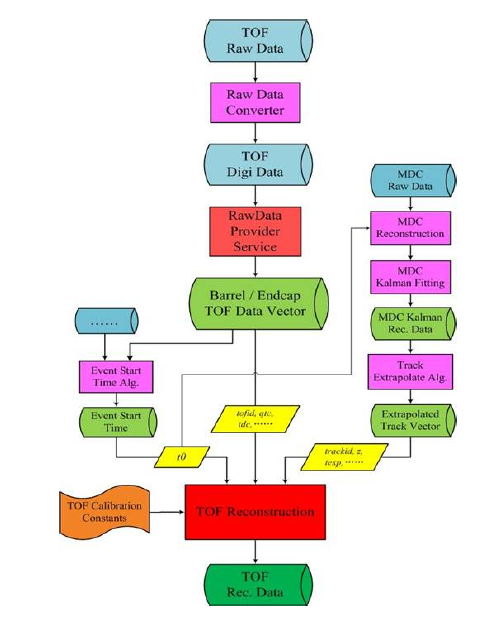
\includegraphics[width=0.6\textwidth]{chap1/TOF-res.png}
  \caption{TOF的离线数据重建过程}
  \label{fig:TOF-res}
\end{figure}

\section{原始数据分布}
图~\ref{fig:digicheck-endcapLeading-east-endcap-histogram}~给出了MRPC端盖TOF的原始的TDC的信息。
\begin{figure}[!h]
  \centering
  \includegraphics[width=0.75\textwidth]{chap1/digicheck-endcapLeading-east-endcap-histogram.eps}
  \caption{原始的TDC}
  \label{fig:digicheck-endcapLeading-east-endcap-histogram}
\end{figure}

图~\ref{fig:T and Q}~给出了~T-Q~匹配后~MRPC~端盖~TOF~的原始的时间和过阈时间的分布。
\begin{figure}[!h]
%\hfill
\begin{minipage}{0.48\linewidth}
  \centerline{ \centering 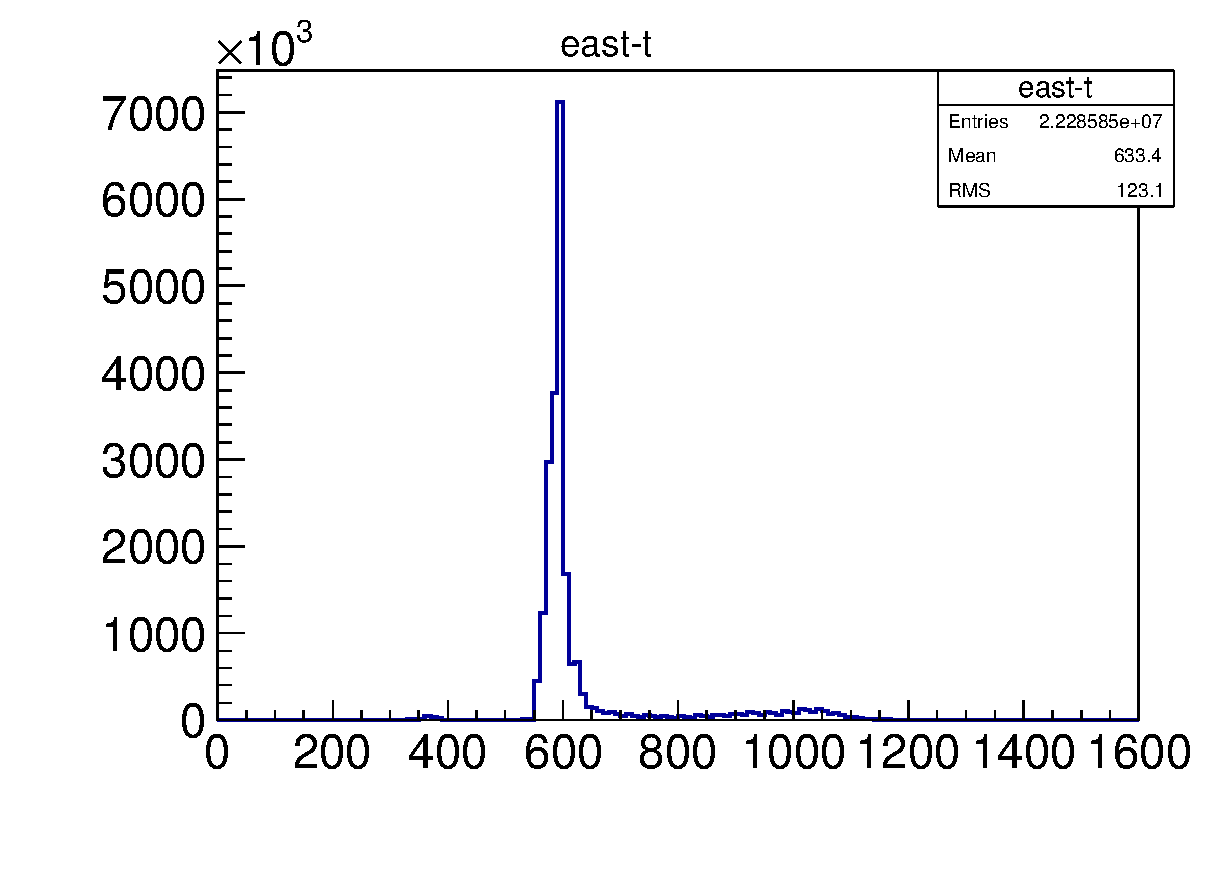
\includegraphics[width=0.75\textwidth]{chap1/endcapcheck-east-t-histogram.eps}}
  \centerline{(a) 东端的原始时间}
  \centerline{\label{fig:endcapcheck-east-t-histogram}}
\end{minipage}
%\hfill
\begin{minipage}{0.48\linewidth}
  \centerline{ \centering 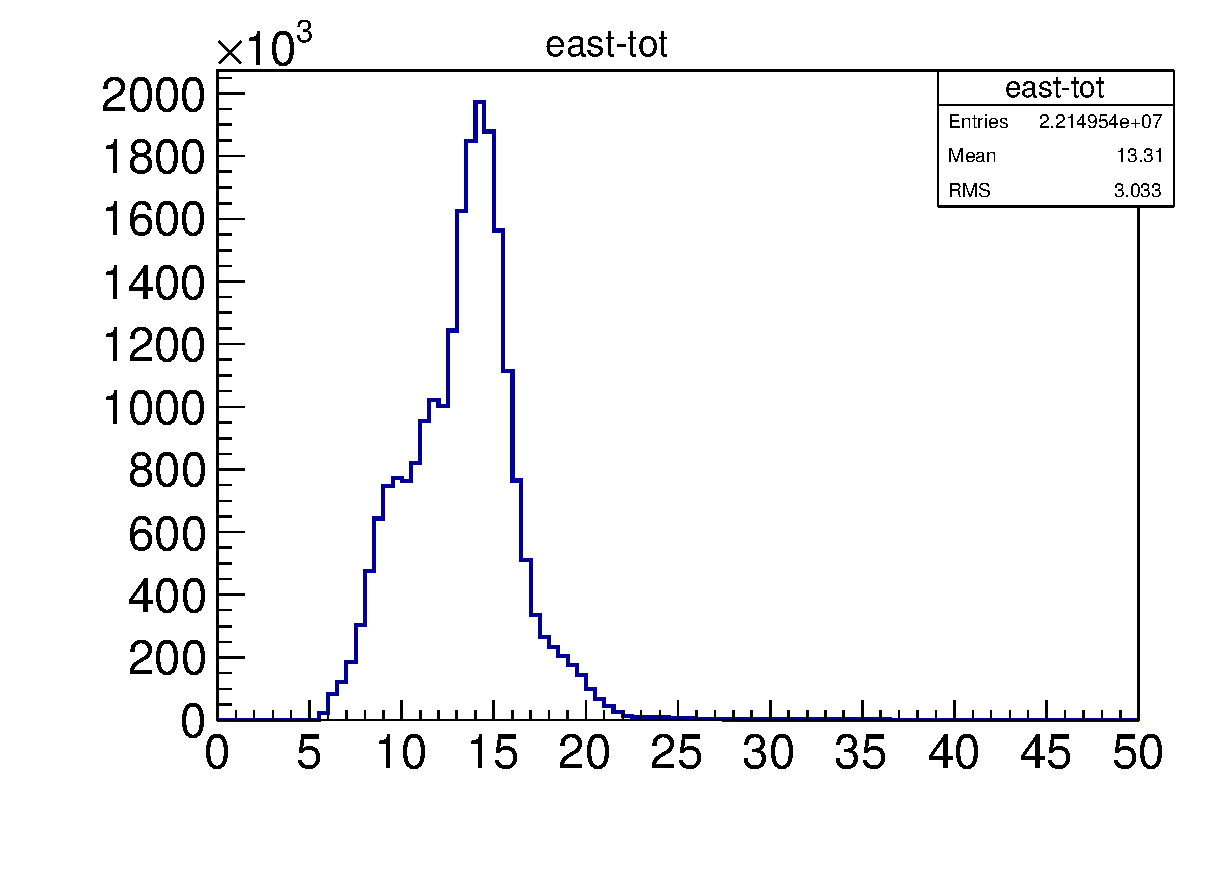
\includegraphics[width=0.75\textwidth]{chap1/endcapcheck-east-tot-histogram.eps}}
  \centerline{(b) 东端的原始TOT}
  \centerline{\label{fig:endcapcheck-east-tot-histogram}}
\end{minipage}
\vfill
%\hfill
\begin{minipage}{0.48\linewidth}
  \centerline{ \centering  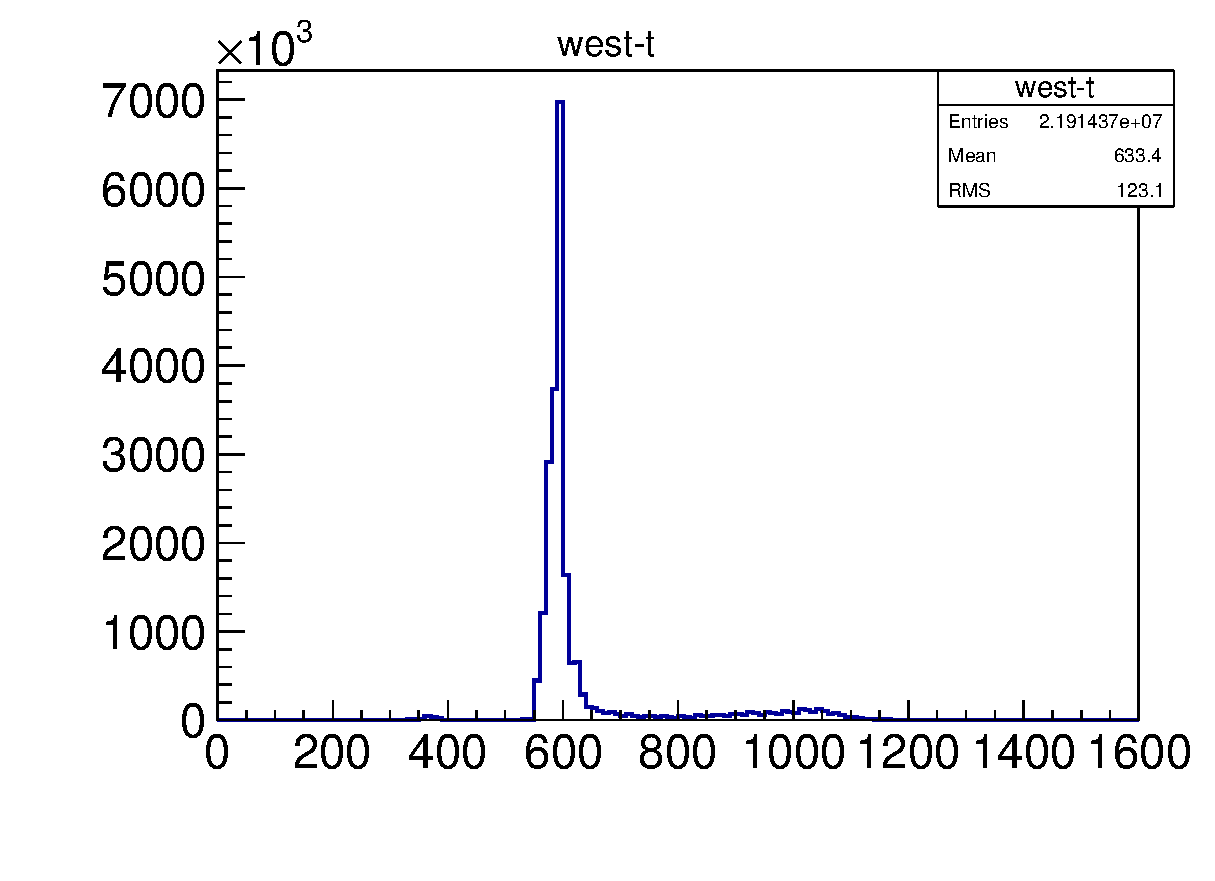
\includegraphics[width=0.75\textwidth]{chap1/endcapcheck-west-t-histogram.eps}}
  \centerline{(c) 西端的原始时间}
  \centerline{\label{fig:endcapcheck-west-t-histogram}}
\end{minipage}
%\hfill
\begin{minipage}{0.48\linewidth}
  \centerline{ \centering 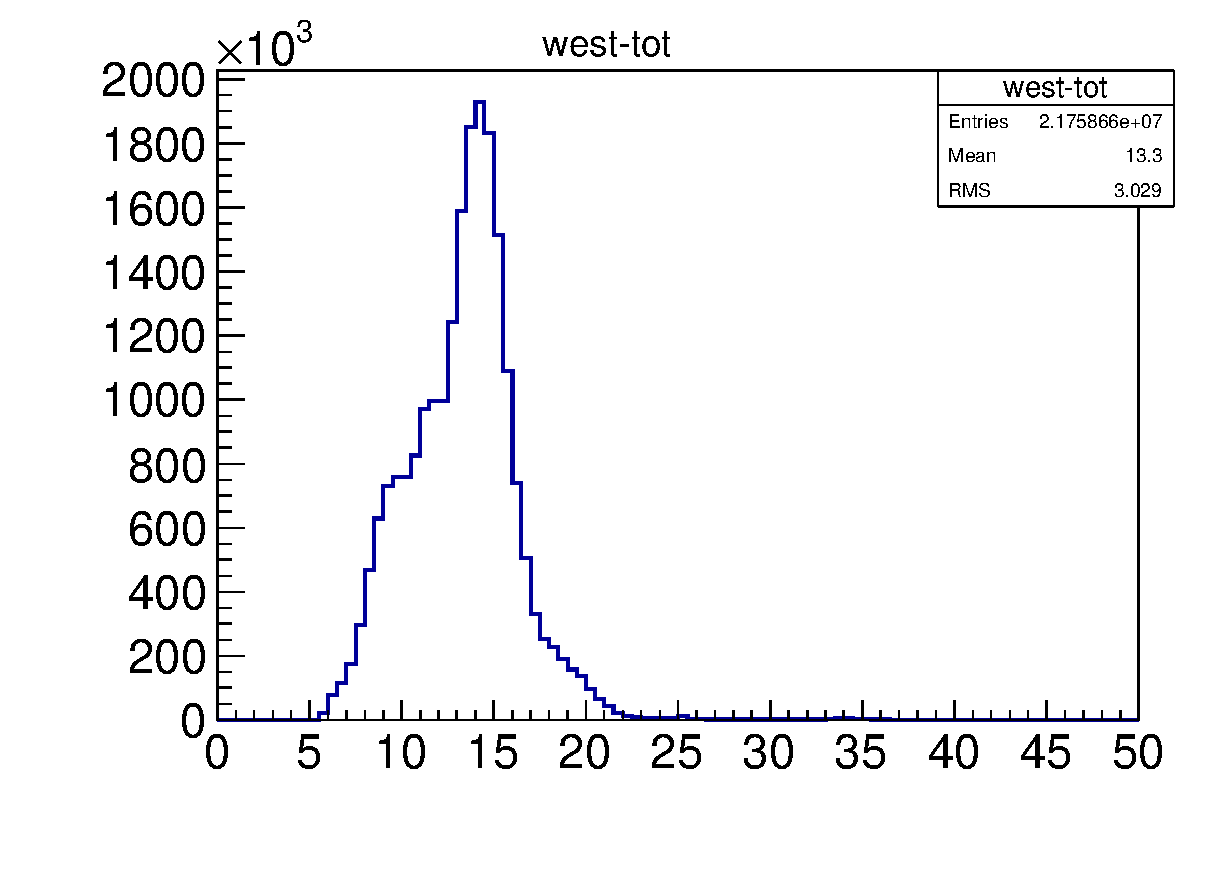
\includegraphics[width=0.75\textwidth]{chap1/endcapcheck-west-tot-histogram.eps}}
  \centerline{(d) 西端的原始TOT}
  \centerline{\label{fig:endcapcheck-west-tot-histogram}}
\end{minipage}
\caption{T-Q匹配后MRPC的原始时间和TOT的分布}
\label{fig:T and Q}
\end{figure}

图~\ref{fig:tofcheck-endcap-est-histogram}~给出了事例起始时间的分布。
\begin{figure}[!h]
  \centering
  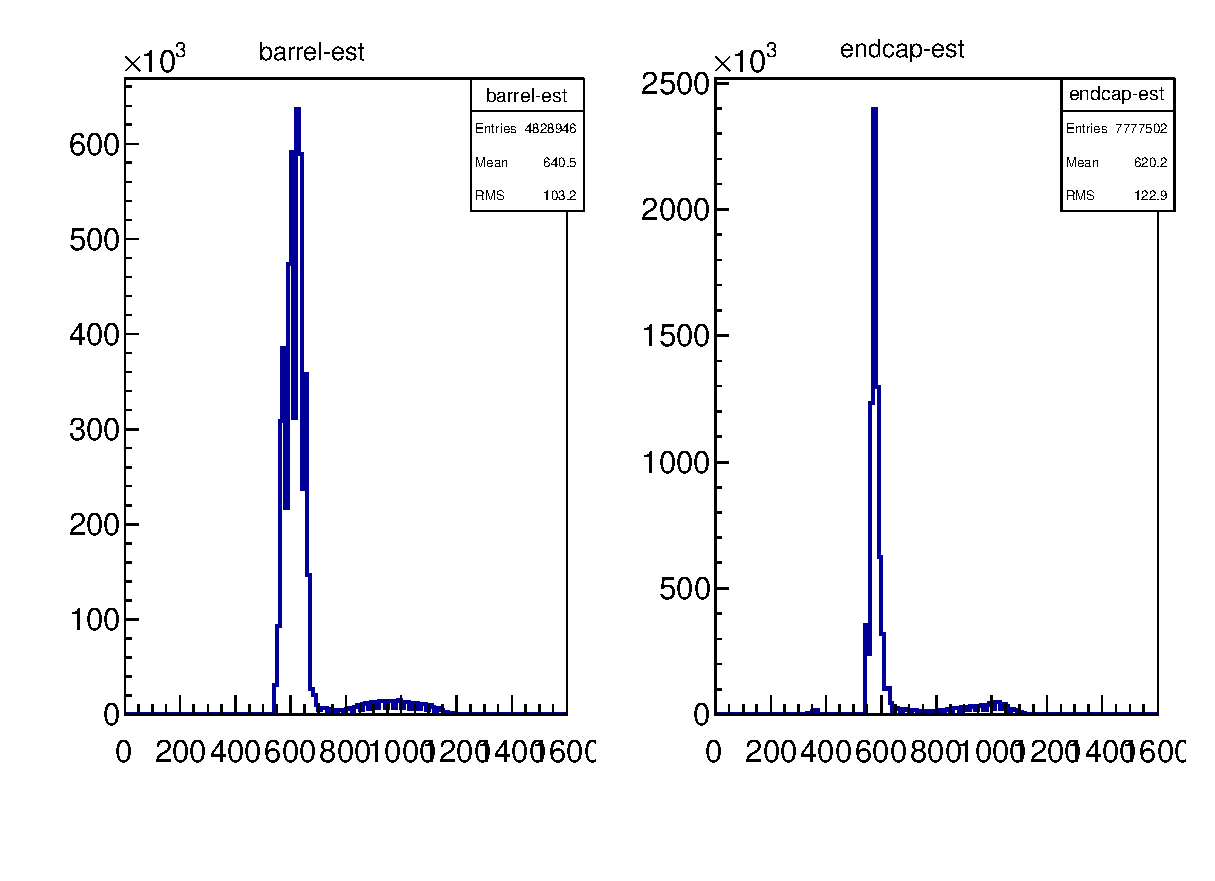
\includegraphics[width=0.9\textwidth]{chap1/tofcheck-endcap-est-histogram.eps}
  \caption{事例起始时间的分布}
  \label{fig:tofcheck-endcap-est-histogram}
\end{figure}

原始测量的时间信号~TDC~包括事例的起始时间~$t_{0}$~,对撞事例从对撞顶点到~TOF~探测器的飞行时间~$t_{tof}$~,信号在读数条的传播时间~$t_{pro}$~,电子学的延迟~$t_{ele}$~,过阈时间的晃动~$t_{time-walk}$~。即:~TDC=$t_{0}$+$t_{tof}$+$t_{pro}$+$_{ele}$+$t_{time-walk}$~,所以飞行时间~$t_{tof}$=TDC-($t_{0}$+$t_{pro}$+$_{ele}$+$t_{time-walk}$)~,其中~TDC~是~TOF~探测器测量到的原始时间信号,对于~MRPC~来讲,采用的双端读数,所以一个事例有两个~TDC~时间信号。~$t_{0}$~由事例起始时间算法给出,~$t_{pro}$~对于~MRPC~来说是信号在对数条的传播时间。这个是刻度的主要内容之一。~$t_{ele}$~是电子学延迟项,是一个常数项。~$t_{time-walk}$~对于~MRPC~来说是~TOT~的晃动。
\section{刻度的重点和难点}
\subsection{MRPC~离线刻度的信息量}
前面已经介绍了~MRPC~直接测量的是时间信号~TDC~,还有过阈时间~TOT~。MRPC~的读数条采用的是双端的读出形式。所以对应一个事例测量的有两个时间信号~TDC1,TDC2;有两个过阈时间~TOT1,TOT2。
在这里定义:
\begin{align}
t_{left}=TDC1-t_{0}
\label{eq:tleft}\\
t_{right}=TDC2-t_{0}
\label{eq:2}
\end{align}
则$t_{left}$和$t_{right}$为事例从对撞点时刻到电子学读出的过阈时间前沿的时刻之间的间隔。包括从对撞点飞行到~MRPC~探测器的飞行时间,信号在读数条中的传播时间,信号在电缆等的传播时间,电子学的时延,过阈时间的晃动等部分。

刻度的目的正是修正除了飞行时间外的其它时间的贡献。其中信号在电缆的传播时间和电子学的时延是常数项,信号在读数条的传播时间是一个依赖击中位置的时间量。过阈时间的晃动是和信号的大小有关的量。

BESIII~系统的坐标定义为:正~Z~轴沿着束流方向,水平向东;正~Y~轴指向天空,竖直向上;正~X~轴取水平向北。取对撞点为坐标原点O(0,0,0)。空间某一点P(x,y,z)的方位角定义为直线OP从正X轴沿逆时针在Z—Y平面投影的角度~$\phi$,在端盖~MRPC~中对应的不同模块的编号和相同模块不同的击中位置(来自径迹外推)。OP的极角定义为OP和正Z轴的夹角~$cos\theta$,在端盖~MRPC~中对应的是读数条的编号。

之前已经介绍了利用~MDC~重建和卡曼滤波径拟合可以得到带电径迹的动量和径迹长度的信息,进而可以求出带电粒子的预期飞行时间~$t_{exp}$。

至此,刻度需要的所有相关量已经介绍完了。包括电子学系统测量的量:初始时间~$t_{left}$,$t_{right}$~(TDC扣除$t_{0}$后的时间在本论文中仍旧称为初始时间),过阈时间~qleft,qright~(测量的两个过阈时间的值在本文中都表示成~qleft,qright~的形式);外推的量:击中位置~zrhit,预期时间~$t_{exp}$,以及模块的编号,读数条的编号。
\subsection{MRPC~离线刻度的时间,过阈时间,击中位置等的原始分布}
图~\ref{fig:some-Diagram}~给出了~MRPC~离线刻度的一些原始的分布。上面的三幅图是原始的时间,过阈时间和击中位置分布的一维图,其中~\ref{fig:left-t}~是原始的时间分布;~\ref{fig:left-q}~是原始的过阈时间的分布,可以明显看出,存在多峰现象;~\ref{fig:left-z}~是击中位置的分布,可以看出事例数随着击中位置是分布均匀的。下面三幅图是原始的时间,过阈时间和击中位置相互关系的二维图,其中~\ref{fig:left-tVSz}~表示时间随击中位置的分布,这个关系近似线性,这是刻度的主要项之一;~\ref{fig:left-tVSq}~表示时间随过阈时间的分布,关系分布复杂,这也是刻度的主要项之一;~\ref{fig:left-qVSz}~表示过阈时间和击中位置的分布。

\begin{figure}[htbp]
\begin{minipage}[t]{0.33\linewidth}
%\centering
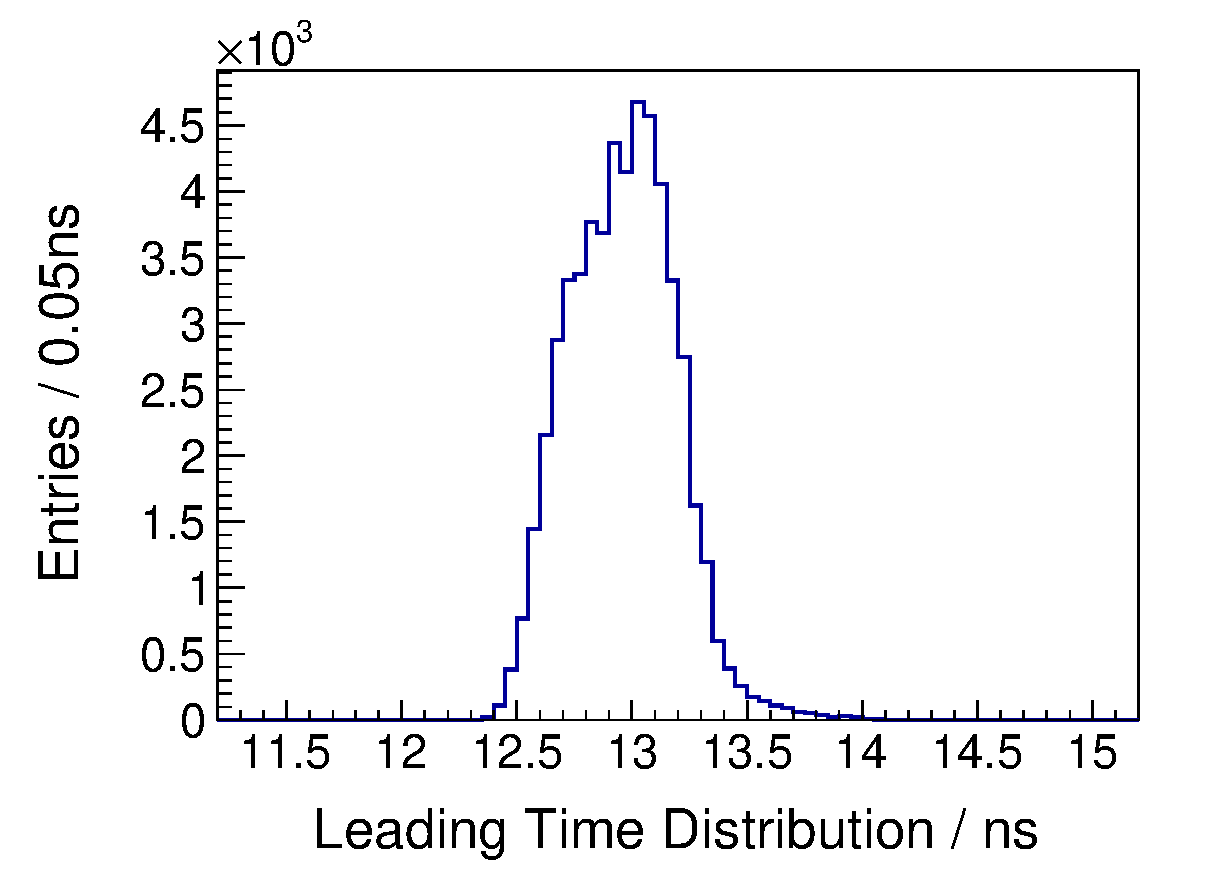
\includegraphics[width=0.9\textwidth]{chap1/left-t.eps}
\subcaption{原始时间的分布}
\label{fig:left-t}
\end{minipage}%
\hfill
\begin{minipage}[t]{0.33\linewidth}
%\centering
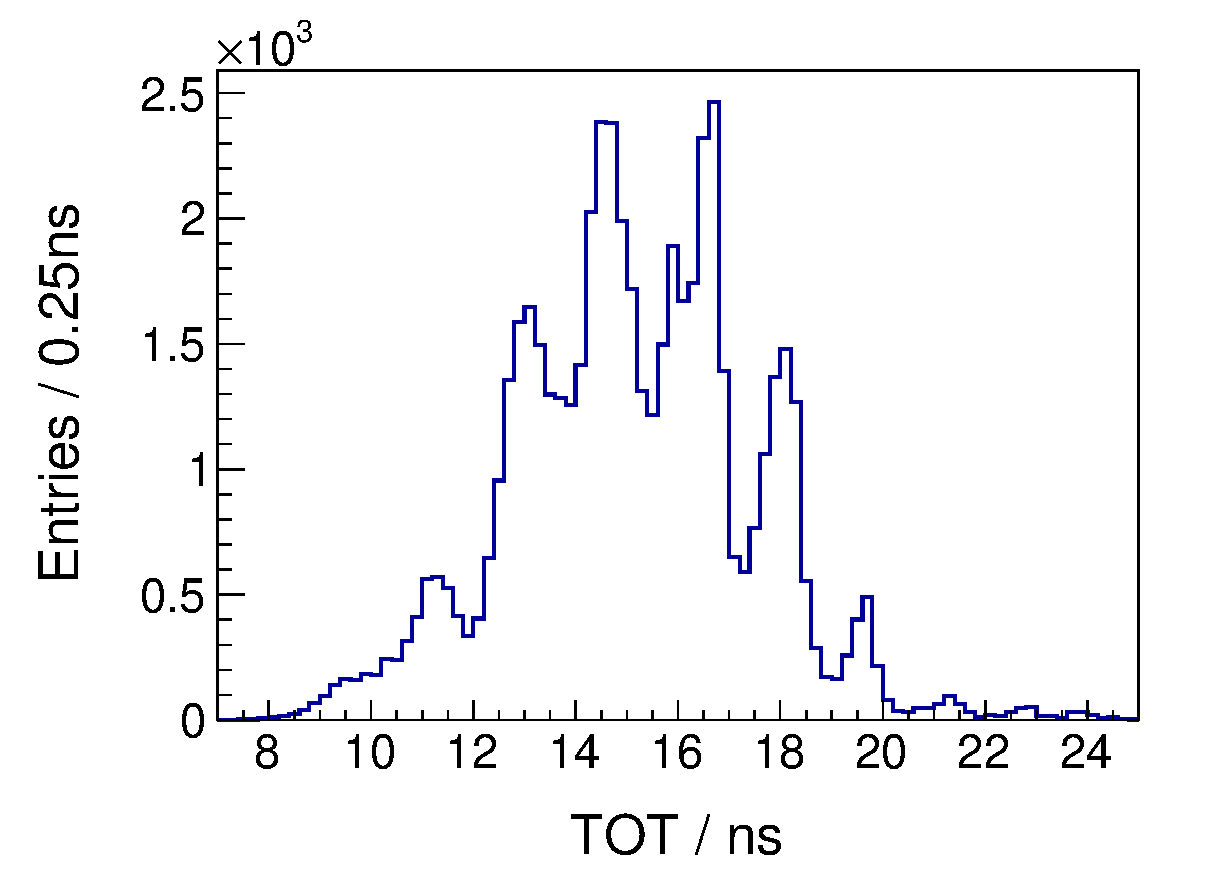
\includegraphics[width=0.9\textwidth]{chap1/left-q.eps}
\subcaption{过阈时间的分布(多峰)}
\label{fig:left-q}
\end{minipage}
\hfill
\begin{minipage}[t]{0.33\linewidth}
%\centering
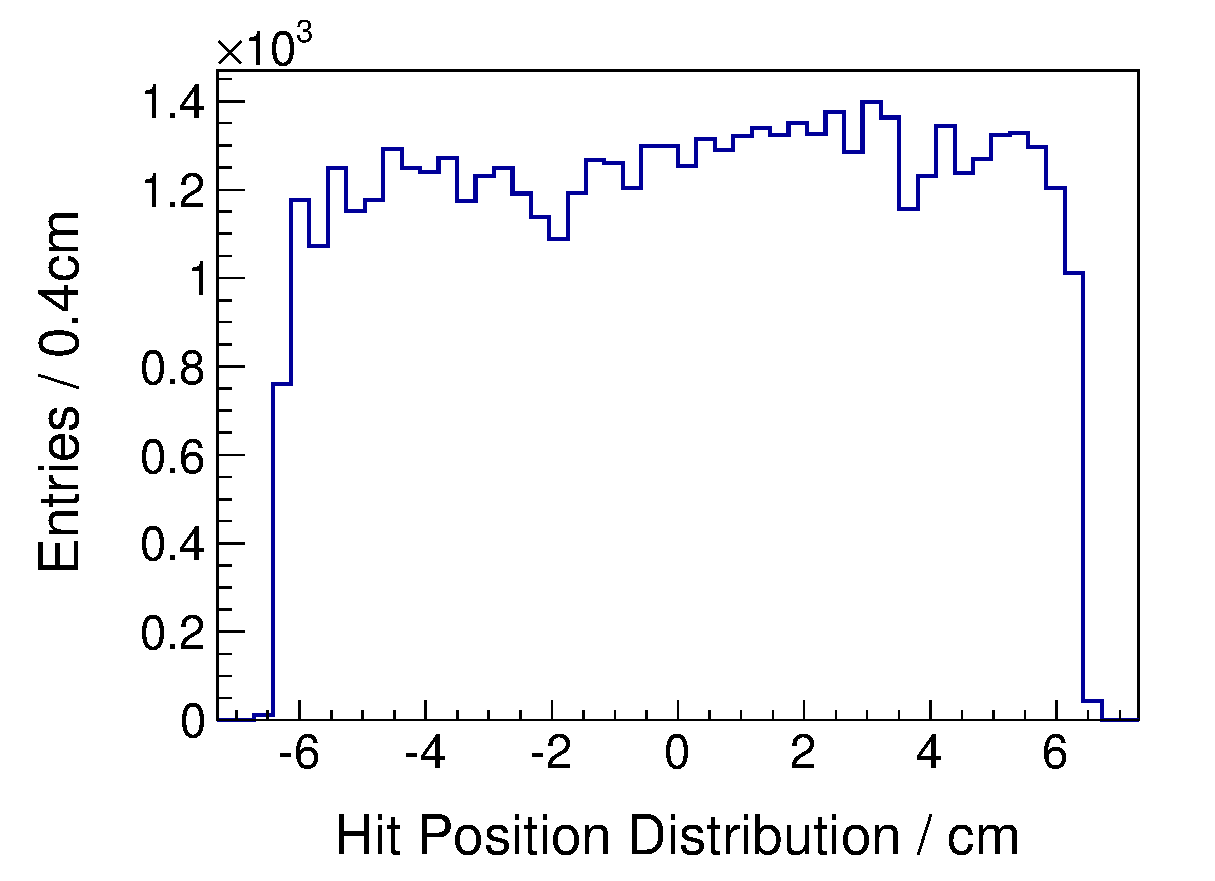
\includegraphics[width=0.9\textwidth]{chap1/left-z.eps}
\subcaption{击中位置的分布}
\label{fig:left-z}
\end{minipage}
\vfill
\begin{minipage}[t]{0.33\linewidth}
%\centering
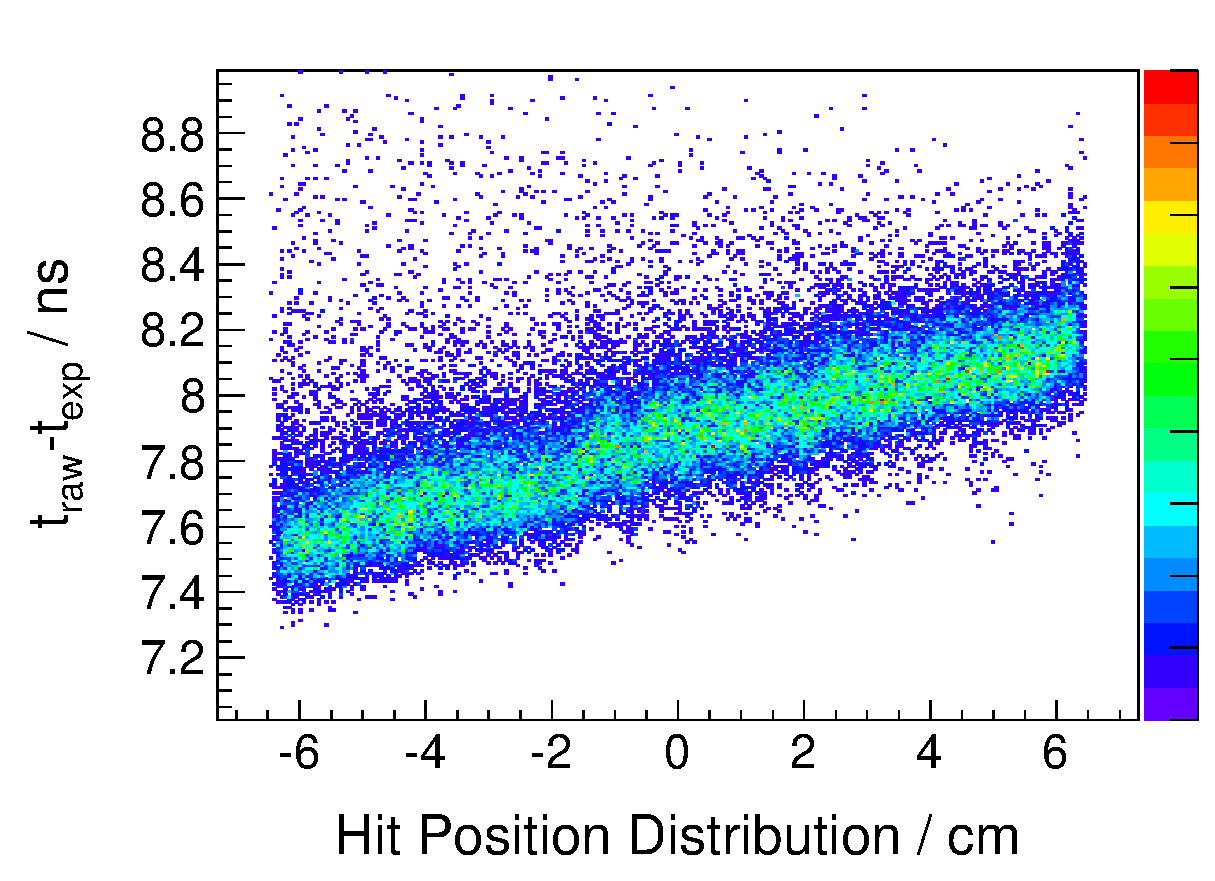
\includegraphics[width=0.9\textwidth]{chap1/left-tVSz.eps}
\subcaption{时间随击中位置的分布}
\label{fig:left-tVSz}
\end{minipage}%
\hfill
\begin{minipage}[t]{0.33\linewidth}
%\centering
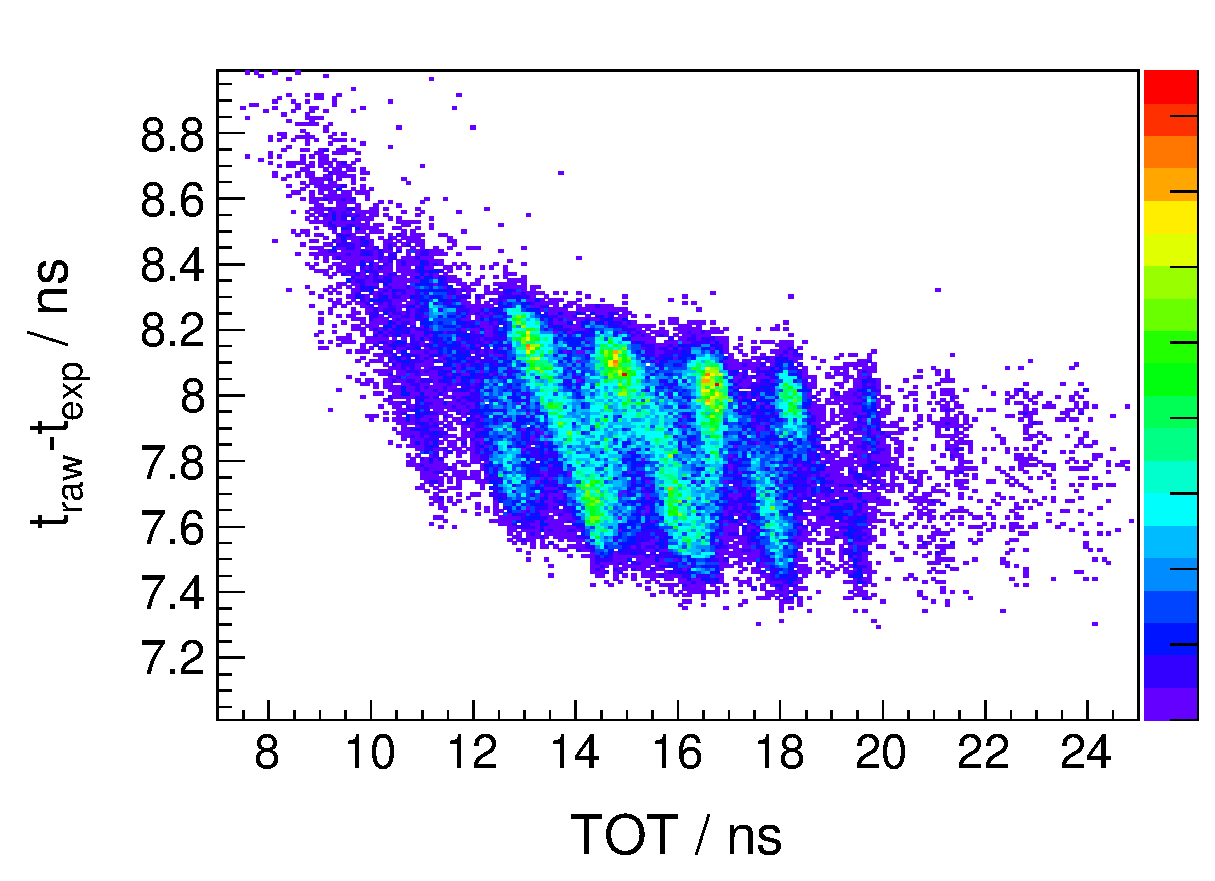
\includegraphics[width=0.9\textwidth]{chap1/left-tVSq.eps}
\subcaption{时间随过阈时间的分布}
\label{fig:left-tVSq}
\end{minipage}
\hfill
\begin{minipage}[t]{0.33\linewidth}
%\centering
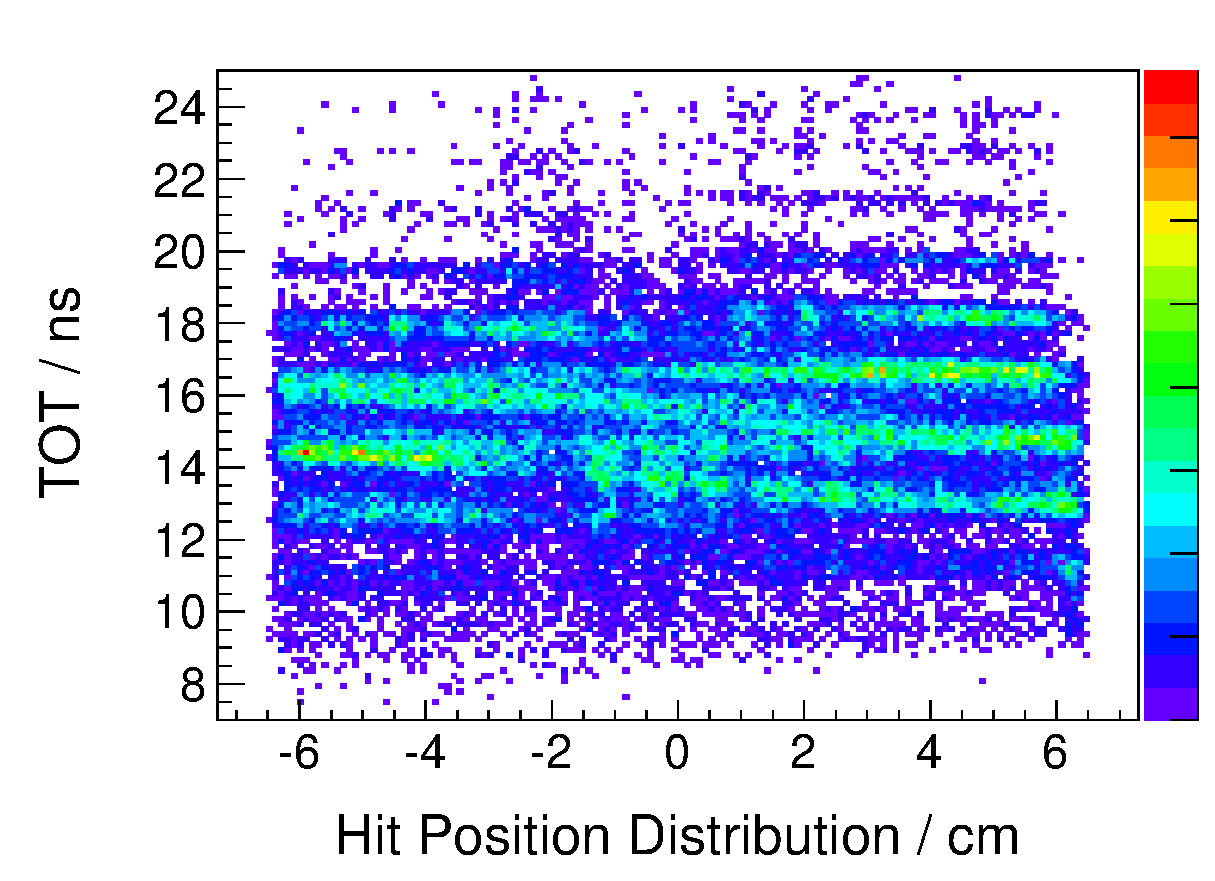
\includegraphics[width=0.9\textwidth]{chap1/left-qVSz.eps}
\subcaption{过阈时间随击中位置的分布}
\label{fig:left-qVSz}
\end{minipage}
\caption{一些原始的分布}
\label{fig:some-Diagram}
\end{figure}

%束团在对撞点发生对撞,产生的次级带电粒子的速度大小和方向在各向都是同性的。
\subsection{过阈时间和反射问题}
刻度的主要内容包括:信号在读数条的传播时间项,过阈时间的修正项。

其中信号在读数条的传播时间和信号在读数条的击中位置以及信号在读数条的等效传播速度有关。对于MRPC的每条读数条而言,长度以及工艺上的差别,导致信号在每个读数条的等效速度不尽相同,因此需要分别对每条读数条进行离线刻度。

信号在读数条的传播时间项如图~\ref{fig:left-tVSz}~所示,近似是一个线性的关系。预估采用低阶多项式即可完成修正。而过阈时间修正项如图~\ref{fig:left-tVSq}~所示,可以看出时间对过阈时间的分布存在折线关系,分布复杂,需要分析这种折线分布背后的产生的机制。采用合适的方式处理这种关系。

\begin{figure}[!h]
\begin{minipage}[!h]{0.5\linewidth}
%\centering
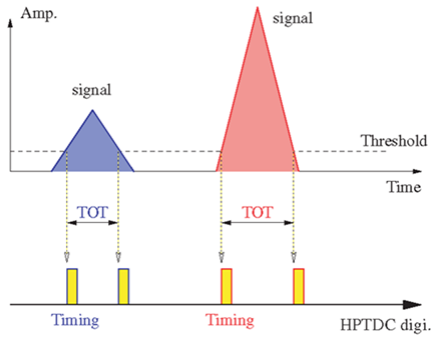
\includegraphics[width=0.8\textwidth]{chap1/TOT.png}
\subcaption{过阈时间~\cite{Shao:2009aa}~}
\label{fig:TOT}
\end{minipage}
\hfill
\begin{minipage}[!h]{0.5\linewidth}
%\centering
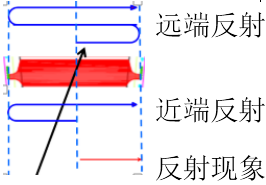
\includegraphics[width=0.9\textwidth]{chap1/reflection.png}
\subcaption{反射问题}
\label{fig:reflection}
\end{minipage}%
\caption{反射问题和过阈时间}
\end{figure}


图~\ref{fig:TOT}~是信号的过阈时间。对于一定的阈值,幅度大小不同的信号,对应的过阈时间不同。信号幅度越大,过阈时间也就越大。
图~\ref{fig:left-q}~中~TOT~的多峰来自于反射。
图~\ref{fig:reflection}~是~MRPC~读数条的反射问题,分为近端反射和远端反射。由于读数条本身较短,反射信号只是比真实信号时间晚不到2ns,这样导致反射信号和原来的真实信号叠加。测量的过阈时间也就变大了。
正是由于过阈时间和反射问题的存在,导致时间对过阈时间的分布复杂。对时间和过阈时间的关系的研究也刻度研究的重点和难点部分。

关于反射和过阈时间有以下结论:
\begin{itemize}
\item{TOT不随击中位置变化}
\item{近端反射是两倍读出条长传播时间。对击中读出条位置没有依赖。}
\item{远端反射依赖击中位置,且与时间依赖关系相反。}
\item{对多次反射的情况,无论近端还是远端反射,相互之间差两倍读出条长的传播时间。}
\end{itemize}

\begin{figure}[!h]
  \centering
  \includegraphics[width=0.9\textwidth]{chap1/TOT-interval.eps}
  \caption{过阈时间的的峰之间的间隔}
  \label{fig:TOT-interval}
\end{figure}
图~\ref{fig:TOT-interval}~表示过阈时间的分布,多峰。两个峰之间的时间间隔是:(19.65ns-11.2ns)/5=1.69ns;

\begin{figure}[!h]
  \centering
  \includegraphics[width=0.9\textwidth]{chap1/TOTvsZ-interval.eps}
  \caption{过阈时间与击中位置图中两个水平线(折线)之间的间隔}
  \label{fig:TOTvsZ-interval}
\end{figure}
图~\ref{fig:TOTvsZ-interval}~表示过阈时间与击中位置的分布。两个水平线之间(近端反射)的时间间隔是:(18.0ns-12.8ns)/3=1.73ns;

读数条编号是~7~的这一条长度是~13~cm,读数条的切角长度是~2.8~cm。信号在读数条传播的等效速度大约是~55~ps/cm(即图~\ref{fig:left-tVSz}~的斜率)。这样信号传播一个读数条长度所需要的时间是:(13+2.8)*55=869ps。传播两倍的读数条长需要的时间是869*2ps=1.738ns。这个值正是对应过阈时间(图~\ref{fig:TOT-interval})之间峰的间隔,和过阈时间与击中位置(图~\ref{fig:TOTvsZ-interval})中两个平行线之间的间隔。

\section{小结}
本章首先介绍了原来的端盖闪烁体~TOF~的时间分辨等性能,由于时间分辨达不到~BESIII~实验高精度测量的要求,端盖~TOF~在~2015~年完成了升级改造,换成了时间分辨更好的~MRPC~探测器。MRPC~探测器作为一种新型的飞行时间探测器,具有时间分辨好,探测效率高,造价便宜等优势。之后介绍了~BESIII~实验的~MRPC~的结构。分东西端盖两部分,各有36个模块。每个模块有12个读数条,采用双端电子学读出信号。BESIII~的离线数据处理和分析系统可以处理包括模拟、刻度、重建和物理分析等一系列的物理问题,其中~BOSS~是整个离线软件的核心。然后介绍了~BESIII~离线数据重建过程,事例起始时间的重建,MDC~的径迹外推,以及~TOF~的离线数据重建过程。最后介绍了~MRPC~端盖TOF的一些原始分布以及刻度的主要内容,MRPC~测量的原始数据是原始的时间和过阈时间。其中原始时间除了包括带电粒子的飞行时间,还有事例起始时间($t_{0}$),信号在读数条内传播的时间,过阈时间的前沿晃动,电缆等的延迟等。这些时间贡献需要刻度修正。其中信号在读数条内的传播时间依赖信号在读数条的有效速度,几乎是一个线性关系。由于反射的原因,导致时间和过阈时间的关系分布复杂。需要采用合适的方式处理。过阈时间的修正也是刻度的重点和难点部分。







